\documentclass{../template/tp}
\usepackage[utf8x]{inputenc}

\usepackage[frenchb]{babel}
\usepackage[T1]{fontenc}

\usepackage{graphicx}
\usepackage{amssymb}
\usepackage{amsmath}
\usepackage{wasysym} %smiley
\usepackage{hyperref}% hyperliens
\usepackage{tikz}
\usetikzlibrary{babel,positioning,calc}
\usepackage[]{circuitikz}
\usepackage{textcomp}
% \usepackage{minted}
\usepackage[long]{datetime}
\usepackage{gensymb} % \ohm, celsius
\usepackage{framed}
\usepackage{pdfpages}
\usepackage{todo}
\usepackage{paralist}

\usepackage{mathastext} % math as standfard text : units are respecting typography conventions.
\usepackage{fancyhdr} %en-tête
\usepackage{qrcode}

% \langexam{frenchb}

\newboolean{koriG}
\ifx\koriG\undefined
\correction{false}
\else
\correction{true}
\fi

% \correction{false}
 %\correction{true}

\author{The Fantastic Four}


%% fancy header & foot
\pagestyle{fancy}
\lhead{[ELEC-H-301] Électronique appliquée\\ TP \no 1 : filtrage et analyse fréquentielle\ifthenelse{\boolean{corrige}}{~-- corrigé}{}}
\rhead{v1.0.2\\ page \thepage}
\cfoot{}
%%

\pdfinfo{
/Author (Raoul Sommeillier, ULB -- BEAMS)
/Title (TP 1 ELEC-H-301, filtrage et analyse fréquentielle)
/ModDate (D:\pdfdate)
}

\hypersetup{
pdftitle={TP 1 [ELEC-H-301] Électronique appliquée : filtrage et analyse fréquentielle},
pdfauthor={Raoul Sommeillier, ©2016 ULB - BEAMS  },
pdfsubject={filtrage et analyse fréquentielle}
}

%\date{\vspace{-1cm}\mydate\today}
%\title{\vspace{-2cm} Labo \no 6\\ Électronique appliquée [ELEC-H-301]\\Réalisation d'un ampli à transistor\ifthenelse{\boolean{corrige}}{~\\Corrigé}{}}

%\author{\vspace{-1cm}}%\textsc{Yannick Allard}}

\setlength{\parskip}{0.5cm plus4mm minus3mm} %espacement entre §
\setlength{\parindent}{0pt}


\begin{document}

\tptitle{}{Séance 1~: Filtrage et analyse fréquentielle}

% \todo{Arranger l'ordre des exercices}
\vspace{-1cm}
%Cette séance d'exercices a pour objectifs de vous apprendre à :
Objectifs : à la fin de cette séance, l'étudiant sera capable de :
\begin{itemize}
\item Identifier la nature d'un filtre
\item Réaliser, lire et interpréter un diagramme de Bode
\end{itemize}
\rule{\linewidth}{.5pt}

%	Exo 4, 6 (+phaseurs example 8.7), 9, 12, 14
%o	Examples
%	 8.7, surtout pour le diagramme des phaseurs  
%o	Exercises : Tous ok sauf 
%	Simulation ? 8.7, 8.10, 8.13, 8.15, 8.20
%	8.16 car besoin 8.15 simulation
%	8.22-26 manquent d’explications

% Q1.2 %%Raoul : j'ai avancé les 2 questions
\Question{
Exprimer une pulsation (ou fréquence angulaire) de $250rad/s$ en fréquence en $Hz$.

\textit{Express an angular frequency of $250rad/s$  as a cyclic frequency (in $Hz$).}
}
{
$$f=\frac{\omega}{2\pi}=39.8Hz$$
}

% Q1.3
\Question{
Exprimer une fréquence de $250Hz$ en pulsation en $rad/s$.

\textit{Express a cyclic frequency of $250Hz$ as an angular frequency (in $rad/s$).}
}
{
$$\omega=2\pi f=1571rad/s$$
}

% Q1.1
\Question{
Calculer la réactance d'un condensateur (ou capacité) de $1\mu F$ à une fréquence de $10kHz$, et la réactance d'une inductance (ou self ou bobine) de $20mH$ à une pulsation de $100rad/s$. Dans chaque cas, inclure les unités dans votre réponse.

\textit{Calculate the reactance of a $1\mu F$ capacitor at a frequency of $10kHz$, and the reactance of a $20mH$ inductor at a frequency of $100rad/s$. In each case include the units in your answer.
}}%
{
$$X_C=\frac{1}{\omega C}=\frac{1}{2\pi fC}=15.9\Omega$$
$$X_L=\omega L=2\Omega$$
}

% Q1.4
\Question{
Considérant que la tension de sortie de ce circuit est aux bornes de la résistance $R_2$, déterminer la fonction de transfert du circuit.

\textit{Determine the transfer function of the following circuit. The output is on $R_2$.}
\begin{center}
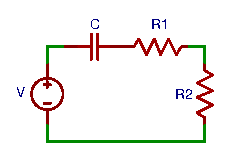
\includegraphics[scale=1.4]{Storey_p166_EX8-4.pdf}
\end{center}
	% \vspace*{-2cm}
	% \marginpar{\qrcode[hyperlink,height=0.5in]{https://easyeda.com/editor\#id=zxbzOkzAm}}
	% \vspace*{2cm}
}
{
$$\frac{\underline{V}_{out}}{\underline{V}_{in}}=\frac{Z_2}{Z_1+Z_2}=\frac{R_2}{R_2+R_1+\frac{1}{j\omega C}}$$
}

% Q1.5
\Question{
Un circuit RC série est formé d'une résistance de $33k\Omega$ et d'un condensateur de $15nF$. Quelle est la constante de temps du circuit ?

\textit{A series RC circuit is formed from a resistor of $33k\Omega$ and a capacitor of $15nF$. What is the time constant of this circuit?}
}
{
$$\tau=RC=495\mu s$$
}

% Q1.6
\Question{
Calculer la constante de temps $\tau$, la pulsation de coupure $\omega_C$ et la fréquence de coupure $f_C$ du circuit RC série suivant\footnote{La plupart des logiciels de CAO éludent le symbole $\Omega$ dans les schémas lors de la spécification des valeurs de résistances. N'oubliez pas de préciser l'unité lorsque vous utilisez des valeurs extraites d'un schéma.}. La sortie est sur la résistance, est-ce un filtre passe-bas ou passe-haut ? %si on précise pas où est la sortie, c'est plus compliqué :-/

\textit{Calculate the time constant $\tau$, the angular cut-off frequency $\omega_C$ and the cyclic cut-off frequency $f_C$ of the following arrangement. Output is on the resistance, is this a high- or a low-frequency cut-off?
}\begin{center}
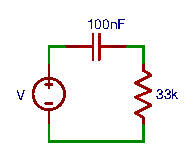
\includegraphics[scale=1.4]{Storey_p167_EX8-6.pdf}
\end{center}
	% \vspace*{-2cm}
	% \marginpar{\qrcode[hyperlink,height=0.5in]{https://easyeda.com/editor\#id=TooWeKARR}}
	% \vspace*{2cm}
}
{
$$\tau=RC=3.3ms$$
$$\omega_C=\frac{1}{\tau}=303rad/s$$
$$f_C=\frac{\omega_C}{2\pi}=48.2Hz$$
C'est un filtre passe-haut ("coupe-bas" ou \textit{low-frequency cut-off} en anglais).
}

% Q1.7
\Question{
Déterminer les fréquences qui correspondent à:
\begin{inparaenum}[(a)]
\item une octave en-dessous de $30Hz$
\item deux octaves au-dessus de $25kHz$
\item trois octaves au-dessus de $1kHz$
\item une décade au-dessus de $1MHz$
\item deux décades en-dessous de $300Hz$
\item trois décades au-dessus de $50Hz$
\end{inparaenum}

\textit{Determine the frequencies that correspond to:
\begin{inparaenum}[(a)]
\item an octave below $30Hz$
\item two octaves above $25kHz$
\item three octaves above $1kHz$
\item a decade above $1MHz$
\item two decades below $300Hz$
\item three decades above $50Hz$
\end{inparaenum}}
}
{
\begin{inparaenum}[(a)]
\item 15 Hz: $15*2^1=30$
\item 100 kHz: $25*2^2=100$
\item 8 kHz: $1*2^3=8$
\item 10 MHz: $1*10^1=10$
\item 3 Hz: $3*10^2=300$
\item 50 kHz: $50*10^3=50000$
\end{inparaenum}
}

% Q1.8
\Question{
Calculer la constante de temps $\tau$, la pulsation de coupure $\omega_C$ et la fréquence de coupure $f_C$ du circuit suivant. La sortie est sur la capacité. Est-ce un filtre passe-bas ou passe-haut ?

\textit{Calculate the time constant $\tau$, the angular cut-off frequency $\omega_C$ and the cyclic cut-off frequency $f_C$ of the following arrangement. The output is on the capacitor. Is this a high- or a low-frequency cut-off.}
\begin{center}
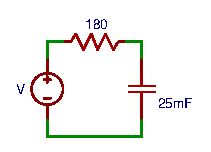
\includegraphics[scale=1.4]{Storey_p167_EX8-9.pdf}
\end{center}
	% \vspace*{-2cm}
	% \marginpar{\qrcode[hyperlink,height=0.5in]{https://easyeda.com/editor\#id=D7LBvOtc9}}
	% \vspace*{2cm}
}
{$$\tau=RC=4.5s$$
$$\omega_C=\frac{1}{\tau}=0.222rad/s$$
$$f_C=\frac{\omega_C}{2\pi}=35.4mHz$$
C'est un filtre passe-bas ("coupe-haut" ou high-frequency cut-off en anglais).
}

% Q1.9
\Question{
Un circuit RL série est formé d'une résistance de $150\Omega$ et d'une inductance de $30mH$. Quelle est la constante de temps de ce circuit ?

\textit{A series RL circuit is formed from a resistor of $150\Omega$ and an inductor of $30mH$. What is the time constant of this circuit?
}}
{
$$\tau=\frac{L}{R}=200\mu s$$
}

% Q1.10
\Question{
Calculer la constante de temps $\tau$, la pulsation de coupure $\omega_C$ et la fréquence de coupure $f_C$ du circuit suivant. La sortie est sur la résistance. Est-ce un filtre passe-bas ou passe-haut ?

\textit{Calculate the time constant $\tau$, the angular cut-off frequency $\omega_C$ and the cyclic cut-off frequency $f_C$ of the following arrangement. The output is on the resistor. Is this a high- or a low-frequency cut-off.}
\begin{center}
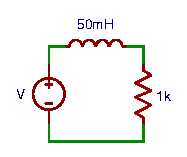
\includegraphics[scale=1.4]{Storey_p167_EX8-12.pdf}
\end{center}
	% \vspace*{-2cm}
	% \marginpar{\qrcode[hyperlink,height=0.5in]{https://easyeda.com/editor\#id=TcF8gQfvL}}
	% \vspace*{2cm}
}
{
$$\tau=\frac{L}{R}=50\mu s$$
$$\omega_C=\frac{1}{\tau}=20000rad/s$$
$$f_C=\frac{\omega_C}{2\pi}=3.18kHz$$
C'est un filtre passe-bas ("coupe-haut" ou \textit{high-frequency cut-off} en anglais).
}

% Q1.11
\Question{
Calculer la constante de temps $\tau$, la pulsation de coupure $\omega_C$ et la fréquence de coupure $f_C$ du circuit suivant. La sortie est sur la self. Est-ce un filtre passe-bas ou passe-haut ?

\textit{Calculate the time constant $\tau$, the angular cut-off frequency $\omega_C$ and the cyclic cut-off frequency $f_C$ of the following arrangement. The output is on the inductor. Is this a high- or a low-frequency cut-off?
}\begin{center}
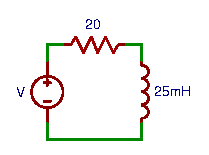
\includegraphics[scale=1.4]{Storey_p168_EX8-14.pdf}
\end{center}
	% \vspace*{-2cm}
	% \marginpar{\qrcode[hyperlink,height=0.5in]{https://easyeda.com/editor\#id=S1Gb6n6N5}}
	% \vspace*{2cm}
}
{
$$\tau=\frac{L}{R}=1.2 ms$$
$$\omega_C=\frac{1}{\tau}=800 rad/s$$
$$f_C=\frac{\omega_C}{2\pi}=127.32Hz$$
C'est un filtre passe-haut ("coupe-bas" ou \textit{low-frequency cut-off} en anglais).
}

% Q1.12
\Question{
Dessiner une approximation asymptotique du diagramme de Bode du circuit des exercices 6, 8, 10 et 11. Utiliser cette approximation pour produire un graphique plus réaliste du gain et de la phase du circuit.

\textit{Sketch a straight-line approximation to the Bode diagram of the circuit of exercises 6, 8, 10 et 11. Use this approximation to produce a more realistic plot of the gain and phase responses of the circuit.}
}
{
Le tracé asymptotique devrait ressembler à celui de la figure 8.13(a) du Storey (ci-dessous à gauche), avec une fréquence de coupure $f_C=199Hz$. La courbe de Bode plus réaliste devrait ressembler à la figure 8.14(a) du Storey (ci-dessous à droite), toujours avec $f_C=199Hz$.

	\begin{minipage}{0.45\linewidth}
		\begin{center}
			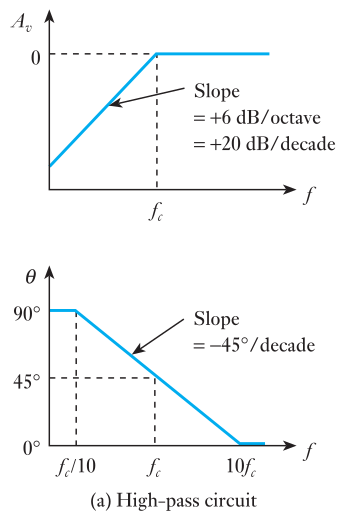
\includegraphics[width=0.9\textwidth]{storey-fig-8-13-a.png}
		\end{center}
	\end{minipage}
	\begin{minipage}{0.45\linewidth}
		\begin{center}
			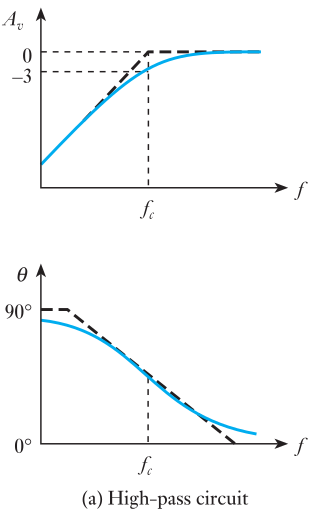
\includegraphics[width=0.8\textwidth]{storey-fig-8-14-a.png}
		\end{center}
	\end{minipage}

}

% Q1.13
\Question{
Un circuit contient trois filtres passe-bas d'ordre 1 et deux filtres passe-haut d'ordre 1. Quels sont les taux de variation du gain de ce circuit à très haute et à très basse fréquences ?

\textit{A circuit contains three high-frequency cut-offs and two low-frequency cut-offs. What are the rates of change of gain of this circuit at very high and very low frequencies?}
}
{
À haute fréquence, le gain va diminuer de $18dB$ par augmentation d'une octave en fréquence (pente de $-18dB/octave$, ou $-60dB/d\acute ecade$). À basse fréquence, le gain va diminuer de $12dB$ par diminution d'une octave en fréquence (pente de $12dB/octave$, ou $40dB/d\acute ecade$).
}

% Q1.14
\Question{
Expliquer ce que signifie le terme \og résonance\fg.

\textit{Explain what is meant by the term ``resonance''.}
}
{
La résonance est discutée en section 8.12 du Storey.
}

% Q1.15
\Question{
Calculer la fréquence de résonance $f_0$, le facteur de qualité $Q$ et la bande passante $B$ du circuit suivant.

\textit{Calculate the resonant frequency $f_0$, the quality factor $Q$ and the bandwidth $B$ of the following circuit.}
\begin{center}
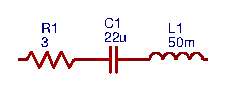
\includegraphics[scale=1.4]{Storey_p168_EX8-19.pdf}
\end{center}
	% \vspace*{-2cm}
	% \marginpar{\qrcode[hyperlink,height=0.5in]{https://easyeda.com/editor\#id=LA6dn33mw}}
	% \vspace*{2cm}
}
{
$$f_0=\frac{1}{2\pi\sqrt{LC}}=152Hz$$
$$Q=\frac{1}{R}\sqrt{\frac{L}{C}}=15.9$$
$$B=\frac{R}{2\pi L}=9.55Hz$$

\begin{center}
	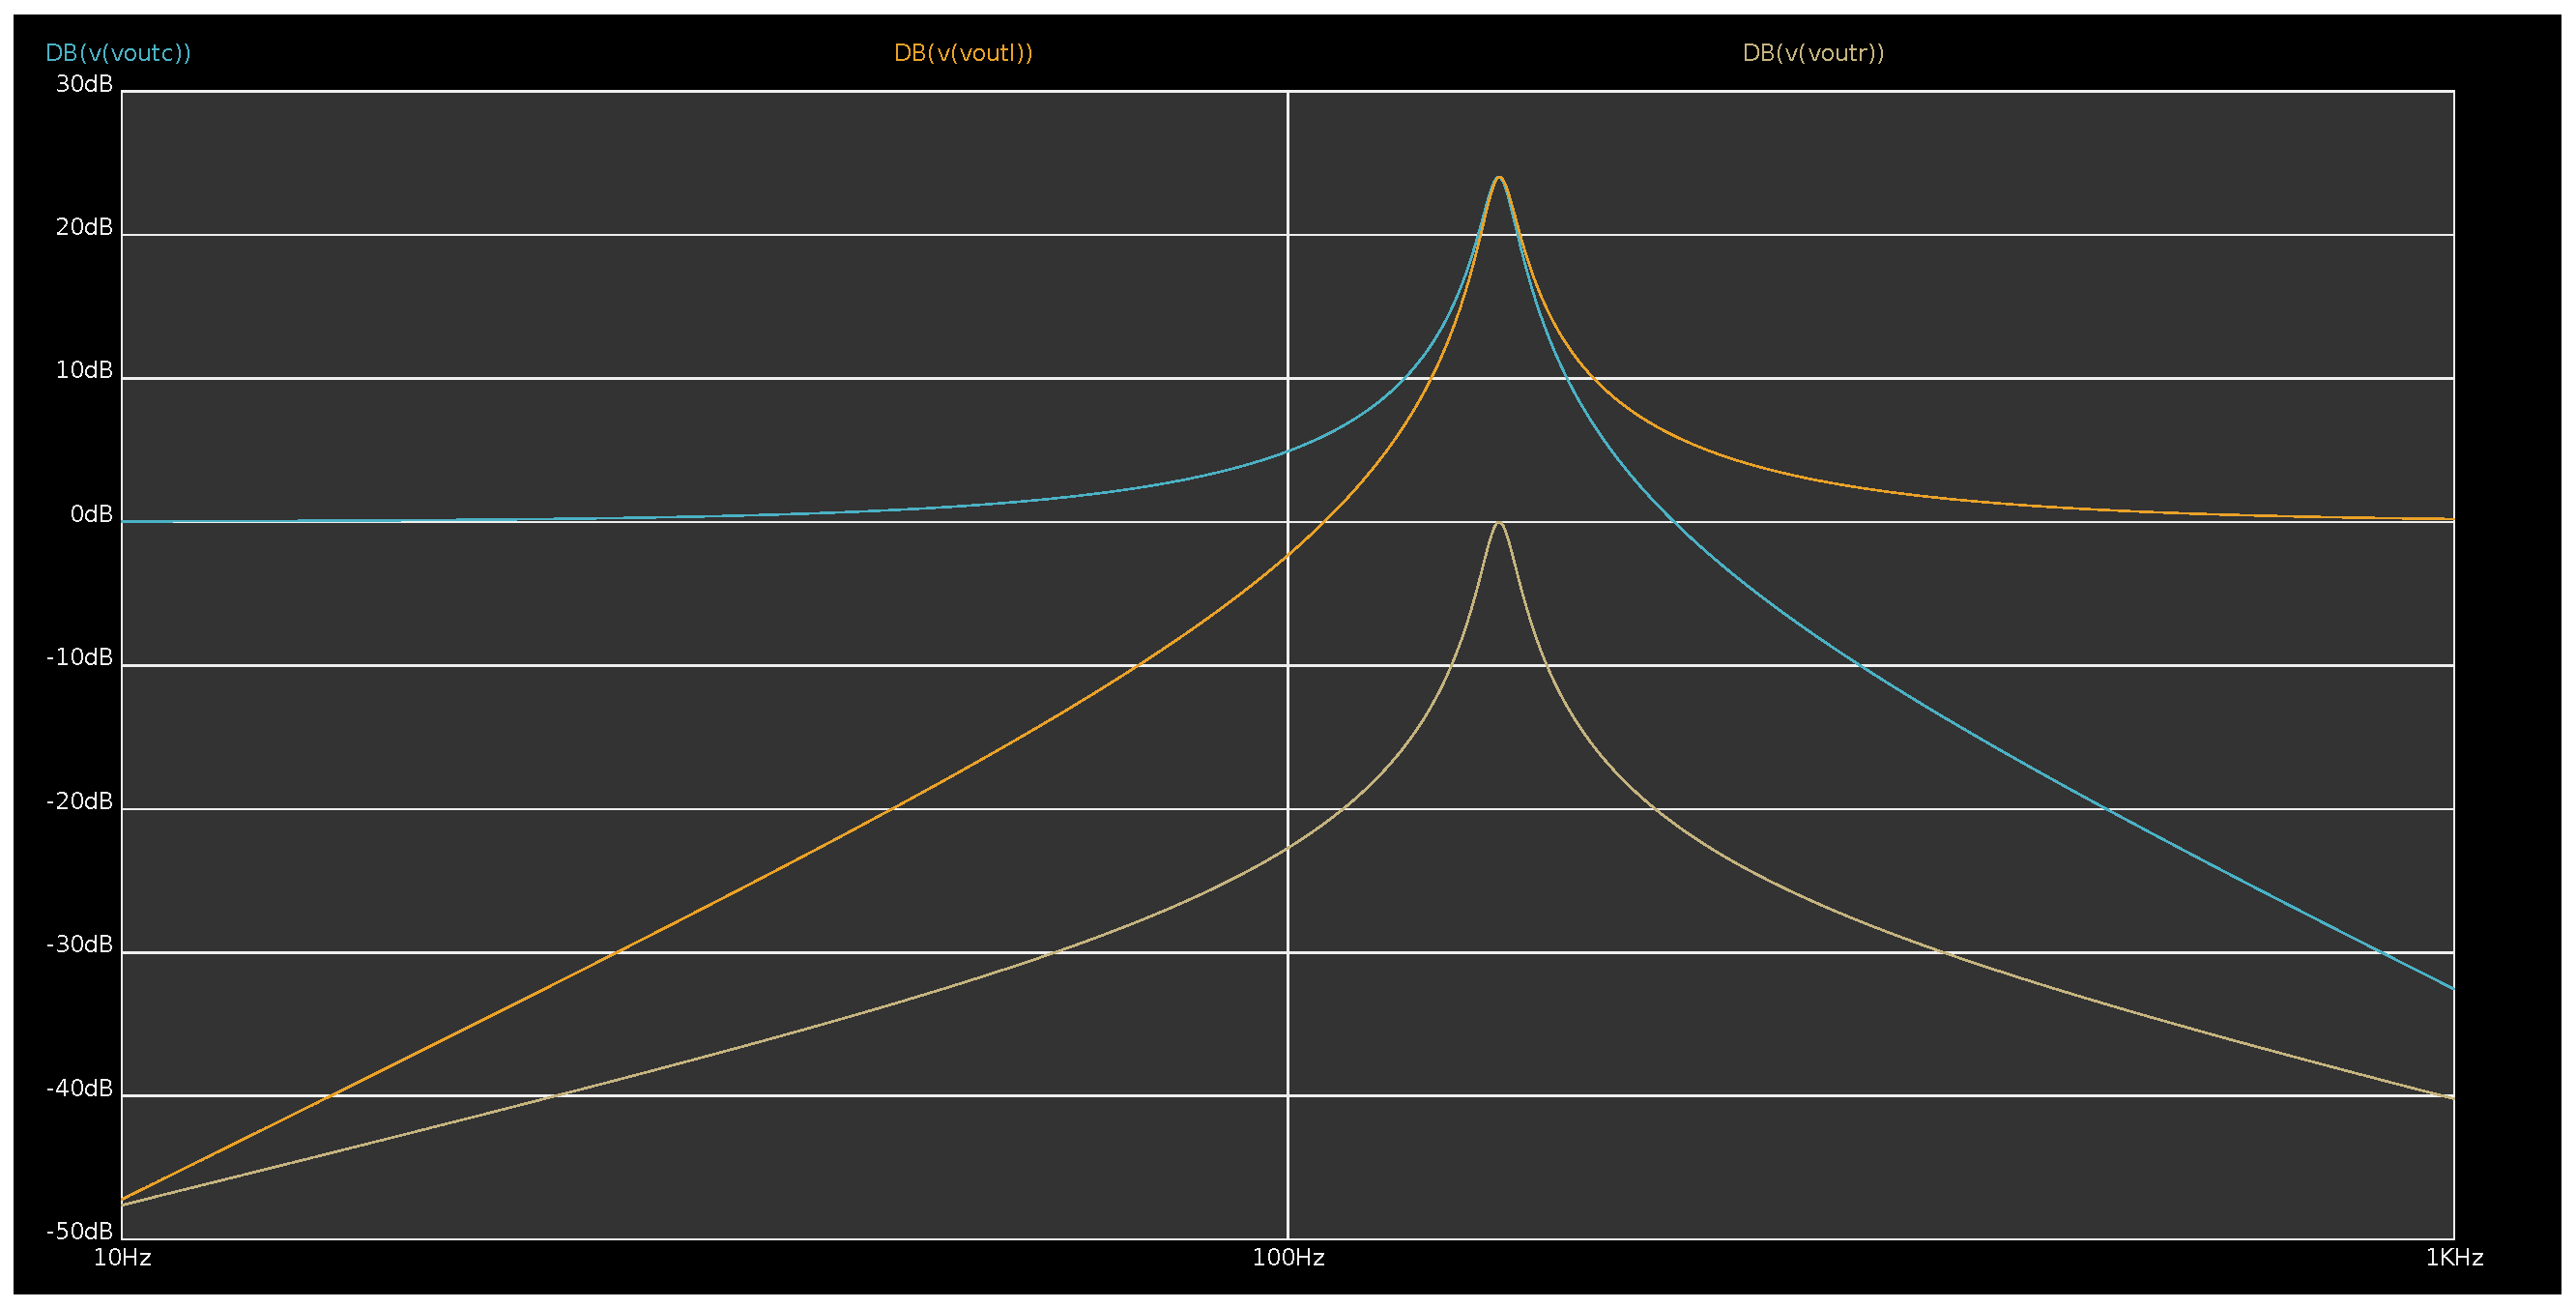
\includegraphics[width=\textwidth]{resonance.pdf}
\end{center}
}

% Q1.16
\Question{
Expliquer la différence entre filtre passif et actif.

\textit{Explain the difference between a passive and an active filter.}
}
{
Les filtres passifs ne contiennent pas de composants actifs, comme par exemple les filtres RL et RC. Les filtres actifs contiennent des composants amplificateurs actifs, comme par exemple un amplificateur opérationnel ou un transistor.
}
% Q1.15
\Question{
Pourquoi les inductances sont souvent évitées dans la construction de filtres ?

\textit{Why are inductors often avoided in the construction of filters?}
}
{
Parce qu'elles sont chères, volumineuses et souffrent de pertes plus conséquentes que les autres composants passifs. De plus elles peuvent être bruyantes et sont sujettes à couplage électromagnétique, avec d'autres inductances du circuit ou avec des champs extérieurs au circuit.
% il ne faut pas oublier que les résistances font 100% de pertes
}
% Q1.15
\Question{
Quel type de filtre actif est optimisé pour produire une réponse fréquentielle plate dans sa bande passante ?

\textit{What form of active filter is optimised to produce a flat response within its pass band?}
}
{
Le filtre de Butterworth. %ou le filtre de Chebyshev de type II
}
% Q1.15
\Question{
Quel filtre est optimisé pour produire une transition nette entre la bande passante et la bande rejetée ?

\textit{What form of active filter is optimised to produce a sharp transition from the pass band to the stop band?}
}
{
Les filtres de Chebyshev.
}
% Q1.15
\Question{
Quel fitre est optimisé pour produite une phase linéaire ?

\textit{What form of filter is optimised for a linear phase response?}
}
{
Le filtre de Bessel est un filtre à phase linéaire.
}
% Q1.15
\Question{
Expliquer pourquoi les capacités parasites et les inductances parasites affectent la réponse en fréquence d'un circuit électronique.
% et les résistances parasites ?

\textit{Explain why stray capacitance and stray inductance affect the frequency response of electronic circuits.}
}
{
Les effets des capacités et inductances parasites sont discutées en Section 8.14 du Storey.
Les effets indésirables sont
\begin{inparaenum}[(a)]
\item pour les capacités parasites: l'introduction de filtres passe-bas dans les circuits, des couplages de signaux entre circuits résultant en de nombreux effets indésirables telle que des interférences (diaphonie ou crosstalk),
\item pour les inductances parasites: l'introduction de filtres passe-bas (par exemple si l'inductance parasite est en série avec une résistance de charge), effet dramatique sur la stabilité des circuits.
\end{inparaenum}
Ces capacités et inductances parasites sont généralement faibles et donc ont tendance à avoir un impact relativement faible à basse fréquence (BF). Cependant, à haute fréquence (HF), elles peuvent avoir des effets dramatiques sur le fonctionnement des circuits. En général, c'est la présence de ces éléments indésirables qui limite les performances à haute fréquence des circuits électroniques.
}

\end{document}
